% Part: sets-functions-relations
% Chapter: infinite
% Section: hilberts-hotel
% Hindi translation (hi-Deva-IN) of Open Logic commit 9620cc73f9c8e0ad003c514a5d3748f29611c4c0.
%
\documentclass[../../../include/open-logic-section]{subfiles}

\begin{document}

\olfileid[hi]{sfr}{infinite}{hilbert}
\olsection{हिल्बर्ट का होटल}

प्राकृत संख्याओं का समुच्चय स्पष्टतः अनंत है। इसलिए यदि हम प्राकृत संख्याओं
को \emph{पहले से उपलब्ध मानकर} नहीं चलना चाहते, तो हमारा पहला कदम ऐसे शब्दों
में अनंत समुच्चय का लक्षण निर्धारित करना होना चाहिए जिनमें स्वयं प्राकृत
संख्याओं का उल्लेख आवश्यक न हो। यहाँ एक सुंदर उपाय है, जिसे हिल्बर्ट ने 1924
के एक व्याख्यान में प्रस्तुत किया। वे हमें यह कल्पना करने को कहते हैं:
\begin{quote}
[\ldots] ऐसे होटल की कल्पना करें जिसमें परिमित संख्या में कमरे हों। इनमें से
हर कमरे में ठीक एक अतिथि ठहरा हो। अब यदि अतिथि किसी तरह अपने कमरे बदल लें,
[पर] इस प्रकार कि हर कमरे में अब भी एक से अधिक व्यक्ति न हो, तो कोई कमरा खाली
नहीं होगा, और होटल-मालिक इस ढंग से नए आने वाले अतिथि के लिए कोई नई जगह नहीं
बना सकता [\ldots
\textparagraph \ldots]

अब हम निर्धारित करते हैं कि होटल में $1$, $2$, $3$, $4$, $5$, \dots, इस प्रकार
अंकित अनंततः अनेक कमरे हों और प्रत्येक में ठीक एक अतिथि ठहरा हो। जैसे ही कोई नया
अतिथि आए, मालिक को बस प्रत्येक पुराने अतिथि को उसके वर्तमान कमरे से एक अधिक
संख्या वाले कमरे में भेजना है; तब कमरा~$1$ नए आए अतिथि के लिए खाली हो जाएगा।
	\begin{center}
		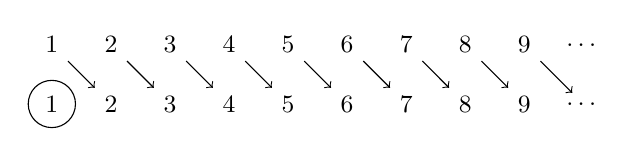
\begin{tikzpicture}[scale = .75]
		\foreach \x in {1, 2, 3, 4, 5, 6, 7, 8, 9}
		{
			\node (\x a) at (\x, 1) {\small{\x}};
			\node (\x b) at (\x, 2) {\small{\x}};
		}
		\node (dotsa) at (10, 1) {\small{\ldots}};
		\node (dotsb) at (10, 2) {\small{\ldots}};
		\draw[->] (1b)--(2a);
		\draw[->] (2b)--(3a);
		\draw[->] (3b)--(4a);
		\draw[->] (4b)--(5a);
		\draw[->] (5b)--(6a);
		\draw[->] (6b)--(7a);
		\draw[->] (7b)--(8a);
		\draw[->] (8b)--(9a);
		\draw[->] (9b)--(dotsa);
		\draw (1,1) circle (.4);
		\end{tikzpicture}
	\end{center}
	(\citealt[730]{EwaldSieg2013} में प्रकाशित; अनुवाद हमारा)
\end{quote}
निर्णायक बात यह है कि हिल्बर्ट के होटल में अनंततः अनेक कमरे हैं; और इस कथन का
क्या अर्थ है, इसे परिभाषित करने के लिए हम उनके विवरण को ग्रहण कर सकते हैं।
वस्तुतः डेडेकिंड का भी यही दृष्टिकोण था (यहाँ उसे, निस्संदेह, बड़े
काल-विपर्यास के साथ प्रस्तुत किया गया है; डेडेकिंड की परिभाषा
\citeyear{Dedekind1888} की है):

\begin{defn}\ollabel{defn:DedekindInfinite}
समुच्चय $A$ \emph{डेडेकिंड-अनंत} है तभी और केवल तभी जब~$A$ से~$A$ के किसी
उचित उपसमुच्चय में कोई !!a{injection} हो। अर्थात् कोई $o \in A$ और कोई
!!a{injection} $f \colon A \to A$ ऐसा है कि $o \notin \ran{f}$।
\end{defn}

\end{document}
